%\section{Cross-Check of Background Prediction Using Full Profiling}
%\label{sec:FullProfiling_Study_Appendix}

%As explained in Section~\ref{sec:htxEVT}, t
The final background 
prediction in the signal region is obtained by fitting two overall
normalization parameters, one for $t\bar{t}$+light jets 
and another for $t\bar{t}$+heavy-flavor jets, to the $\HT$ distribution in the
three analysis channels \chii, \chiii\ and \chiv. 
This simplified background 
calibration may not be sufficient to obtain an accurate 
(both in terms of normalization and shape) 
modeling of the background in the most sensitive channel, the
\chiv\ channel.
In particular, a potential slope in the data to Monte Carlo 
ratio versus $\HT$ would not be corrected for by the 
simple two-parameter fit.

Here we study the predicted background by performing 
a fit to data considering all nuisance parameters 
(a total of 38) describing fundamental
sources of uncertainty in the analysis (referred to as 
``full profiling''). This allows 
to correct for potential mismodelings in the 
background-dominated channels
and port those corrections in a physical way 
into the signal region. 
To be consistent, the nominal $t\bar{t}$ \texttt{ALPGEN} 
prediction, rather than the scaled one, is used.

The results obtained, detailed in Appendix~\ref{app:fullprofiling},
give that most nuisance parameters are well within
$1\sigma$ of their a-priori value (zero) and almost 
not constrained with respect to their a-priori error (one). 
%Prefit & Postfit (full profiling) & Postfit (two-parameter fit) \\
Figure~\ref{fig:HT_SignalRegion_FullProfiling} compares, 
for each of the three analysis channels, the $\HT$ distribution 
prefit and postfit from the fit using full profiling, and with 
the postfit distribution
obtained from the two-parameter fit. As it can be appreciated, 
the full profiling achieves the desired effect of correcting 
the shape of the $\HT$ 
distribution in the low $b$-tag multiplicity channels. However, 
in the $\geq 4$ $b$-tags channel both post-fit predictions still look quite similar,
which gives confidence in the simplified fit procedure.
The corresponding postfit yields after full profiling are 
compared to the yields from the two-parameter fit in
 Appendix~\ref{app:fullprofiling}, and the total background predictions 
in the \chiv\ channel are found to be in agreement within $\sim 10\%$.

\begin{figure}[h!tb]\begin{center}
\begin{minipage}{0.27\textwidth}
\centering
Prefit
\end{minipage}\begin{minipage}{0.27\textwidth}
\centering
Postfit\\ (full profiling)
\end{minipage}
\begin{minipage}{0.27\textwidth}
\centering
Postfit\\ (two-parameters fit)
\end{minipage}
	\subfigure[]{
\includegraphics[width=0.27\textwidth]{htx_analysis_14ifb/figures/fullprof/Prefit/HTAll_6jetin2btagex_ELEMUON.eps}}
	\subfigure[]{
\includegraphics[width=0.27\textwidth]{htx_analysis_14ifb/figures/fullprof/PostFit_null/HTAll_6jetin2btagex_ELEMUON.eps}}
	\subfigure[]{
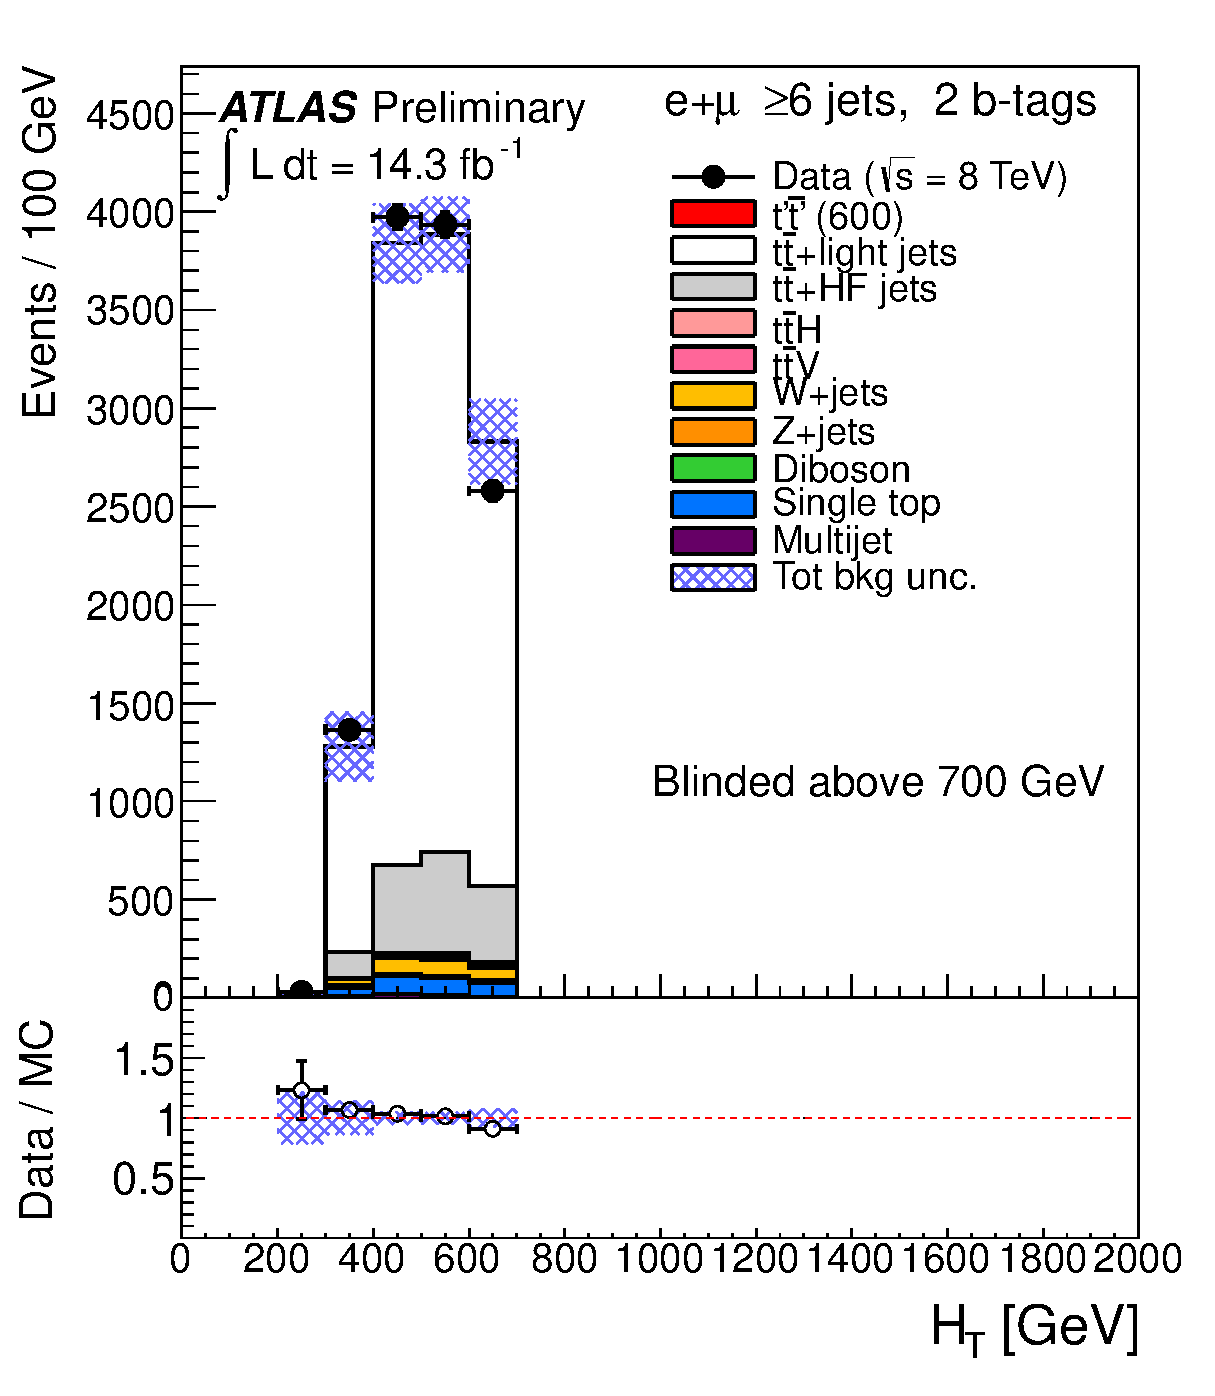
\includegraphics[width=0.27\textwidth]{htx_analysis_14ifb/figures/fullprof/sysband_Postfit_null/HTAll_6jetin2btagex_ELEMUON.eps}} \\
	\subfigure[]{
\includegraphics[width=0.27\textwidth]{htx_analysis_14ifb/figures/fullprof/Prefit/HTAll_6jetin3btagex_ELEMUON.eps}}
	\subfigure[]{
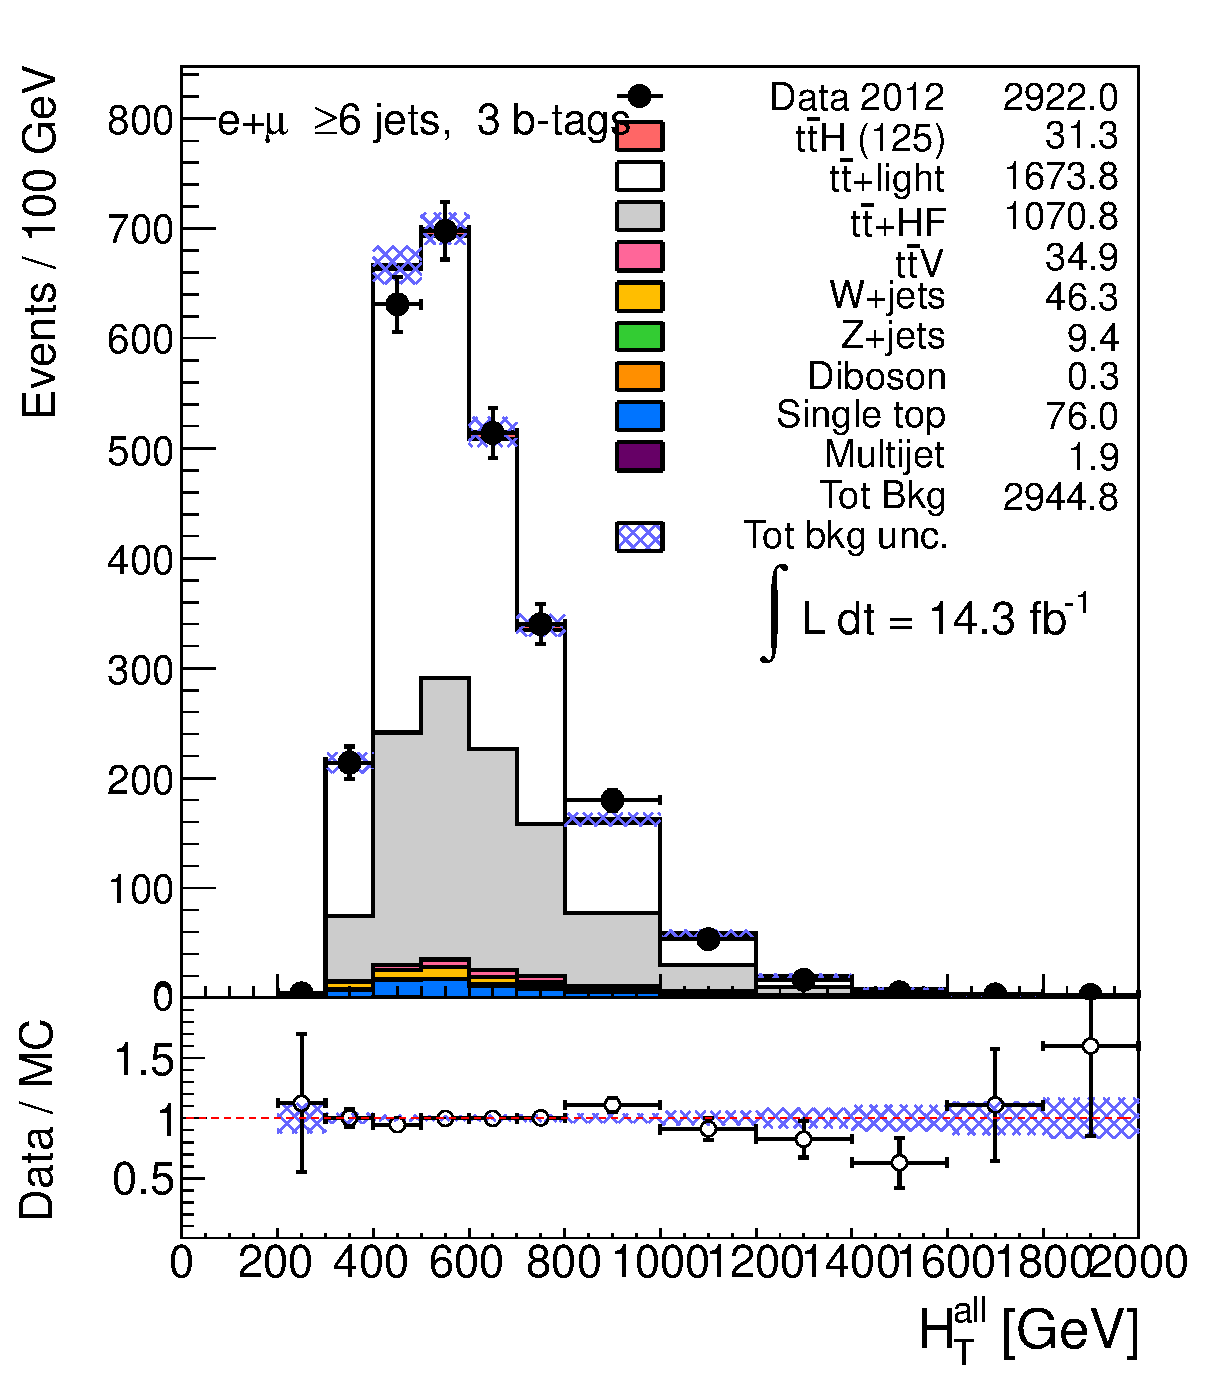
\includegraphics[width=0.27\textwidth]{htx_analysis_14ifb/figures/fullprof/PostFit_null/HTAll_6jetin3btagex_ELEMUON.eps}}
	\subfigure[]{
\includegraphics[width=0.27\textwidth]{htx_analysis_14ifb/figures/fullprof/sysband_Postfit_null/HTAll_6jetin3btagex_ELEMUON.eps}} \\
	\subfigure[]{
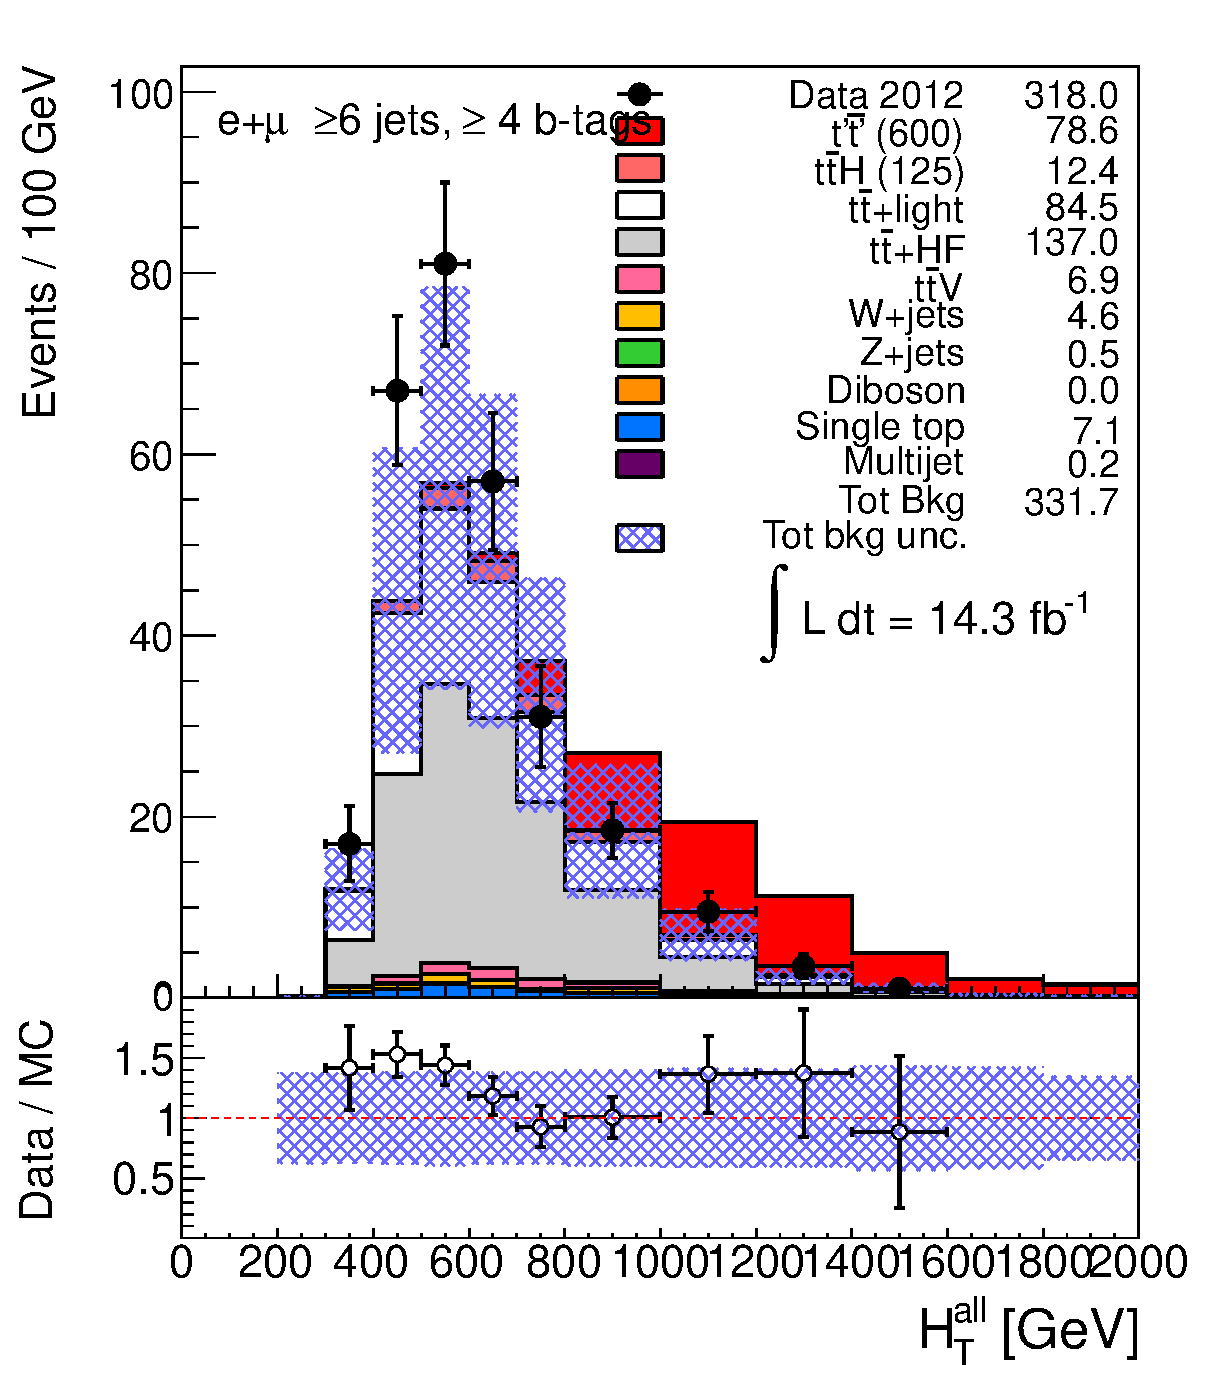
\includegraphics[width=0.27\textwidth]{htx_analysis_14ifb/figures/fullprof/Prefit/HTAll_6jetin4btagin_ELEMUON.eps}}
	\subfigure[]{
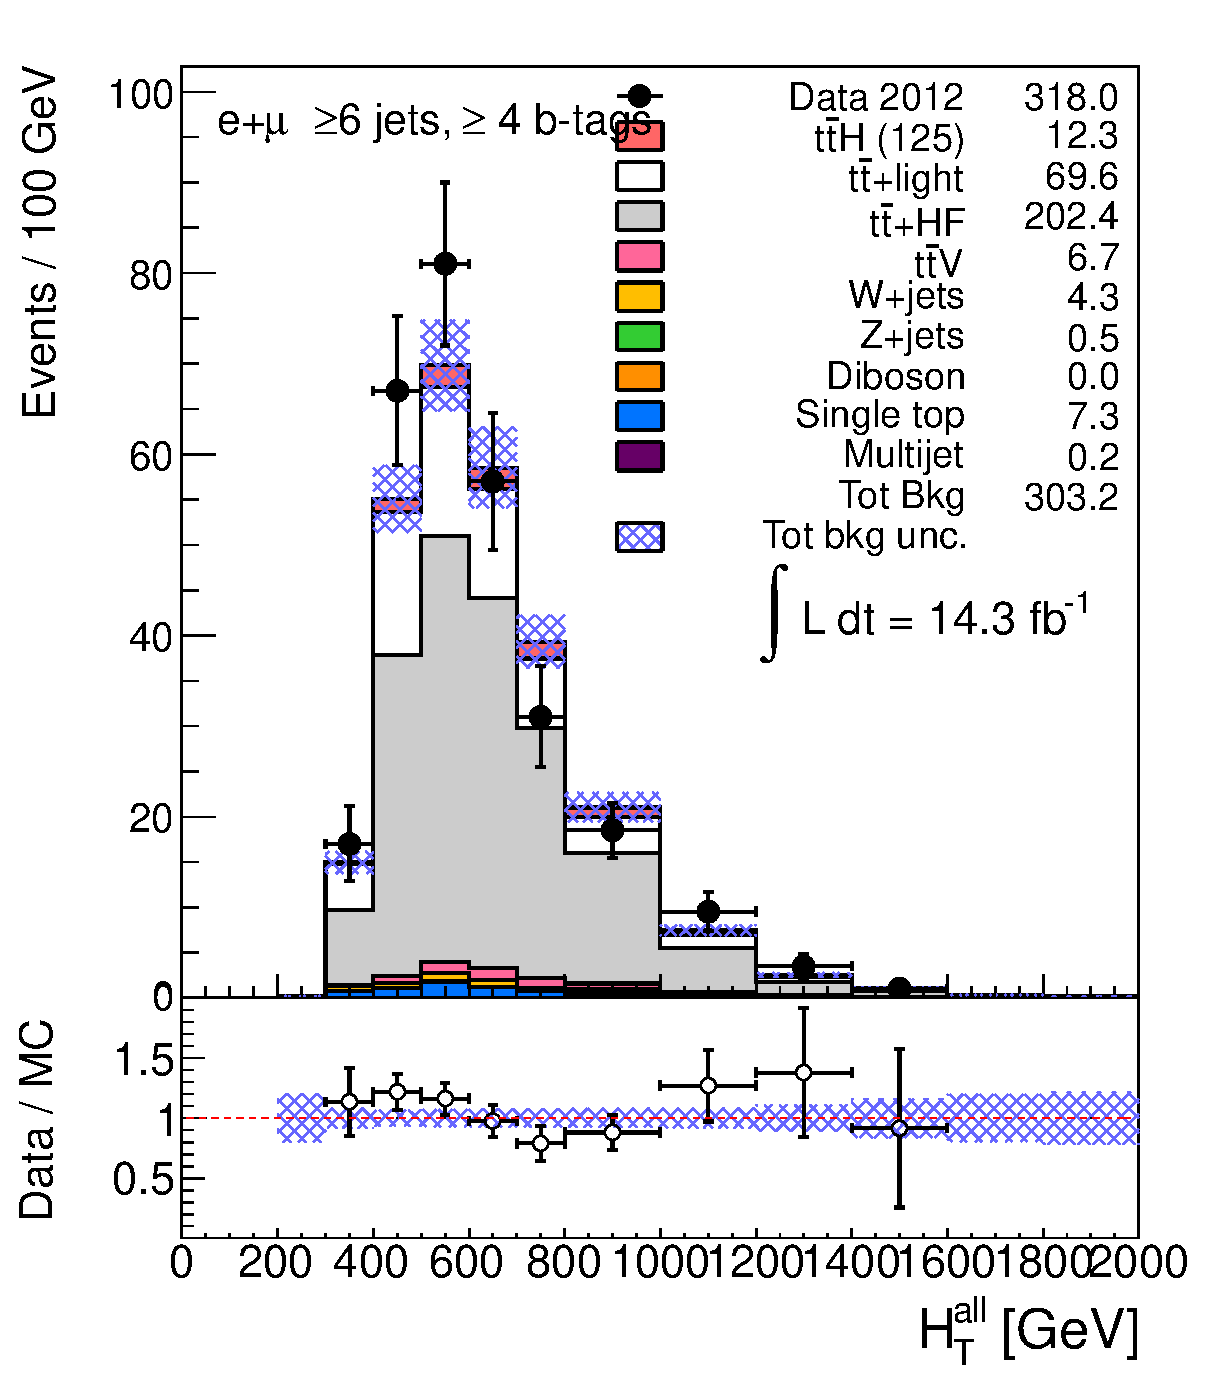
\includegraphics[width=0.27\textwidth]{htx_analysis_14ifb/figures/fullprof/PostFit_null/HTAll_6jetin4btagin_ELEMUON.eps}}
	\subfigure[]{
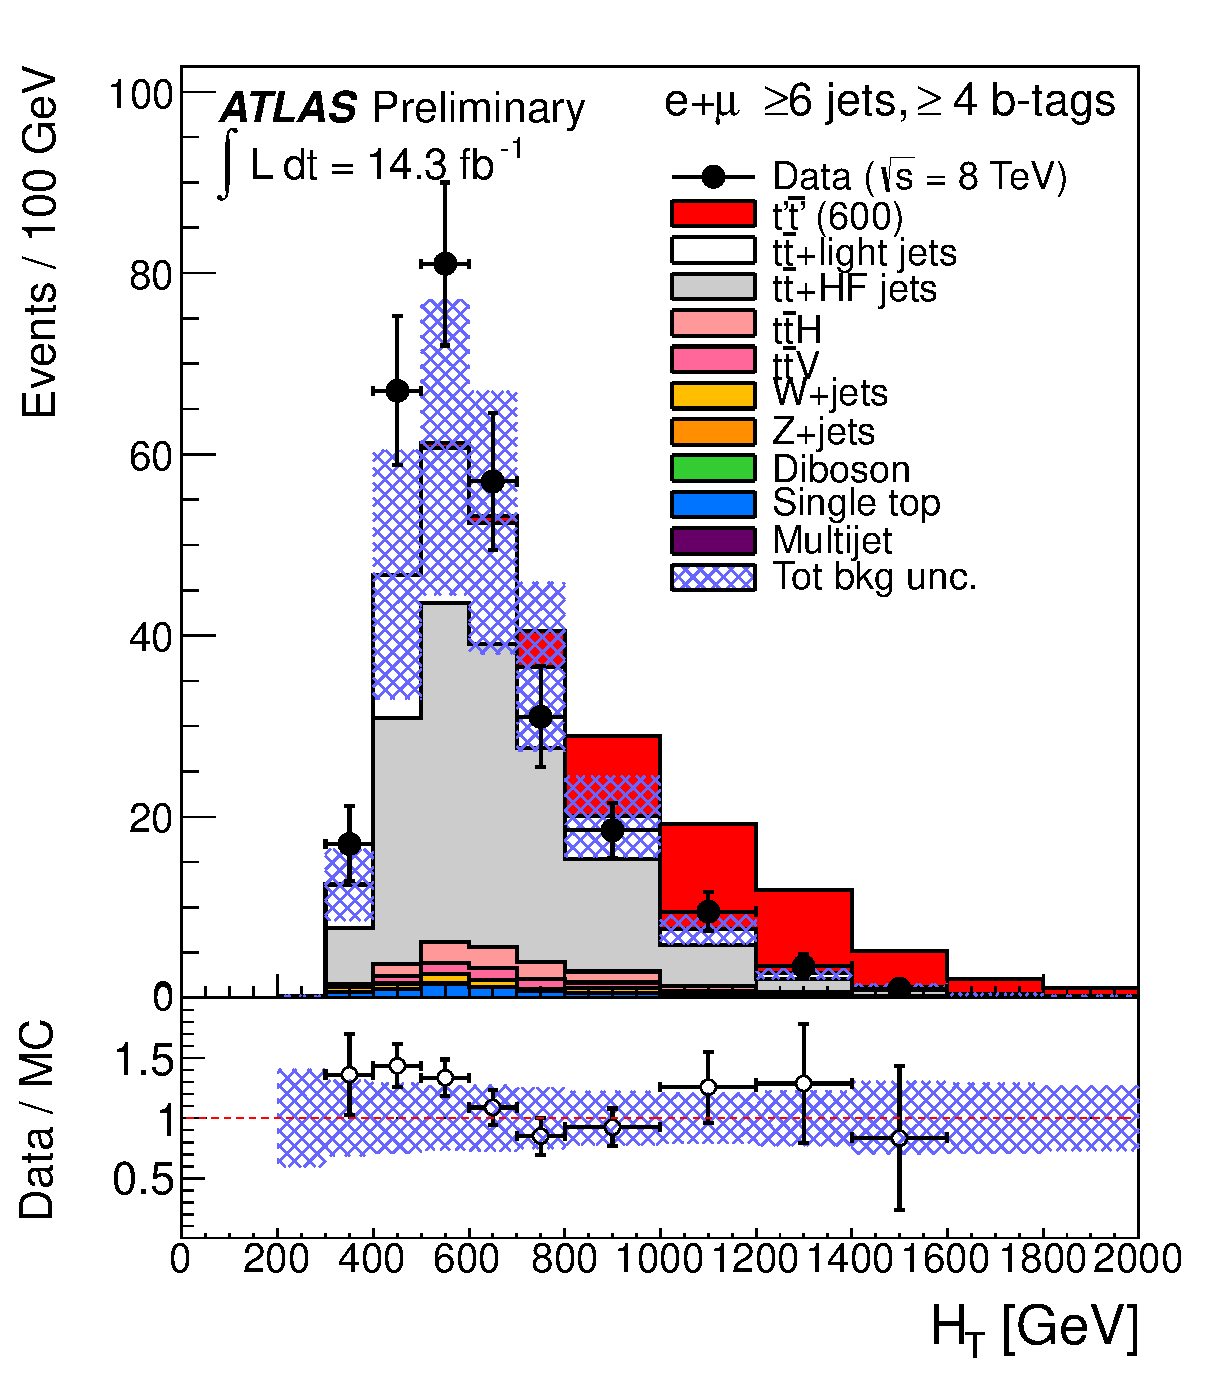
\includegraphics[width=0.27\textwidth]{htx_analysis_14ifb/figures/fullprof/sysband_Postfit_null/HTAll_6jetin4btagin_ELEMUON.eps}} \\
\caption{
Comparison between data and simulation for $\HT$ in the combined
electron and muon channels with $\geq 6$ jets and (a-c) \chii, (d-f) \chiii, and (g-i) \chiv.
From left to right: prefit (nominal $t\bar{t}$ \texttt{ALPGEN} prediction), 
postfit (full profiling of systematic uncertainties) and postfit (two-parameter fit).
The last bin in all figures contains the overflow. The bottom panel displays the ratio between data
and background prediction. The shaded area represents the total post-fit background uncertainty.}
%{\bf Caveat: for the "two-parameter fit" uncertainties are actually still prefit.}}
\label{fig:HT_SignalRegion_FullProfiling}
\end{center}\end{figure}

